\documentclass[11pt]{extarticle}
\usepackage[utf8]{inputenc}
\usepackage{amsmath}
\usepackage{hyperref}
\usepackage[shortlabels]{enumitem}
\usepackage{tikz}
\usepackage{textcomp}

\addtolength{\textwidth}{1.0in}
\addtolength{\textheight}{0.75in}
\addtolength{\evensidemargin}{-0.75in}
\addtolength{\oddsidemargin}{-0.75in}
\addtolength{\topmargin}{-1.0in}

\title{2D Geometry - Answers}
\author{Eric Xiao}
\date{April 2020}

\begin{document}

\maketitle

\begin{enumerate}
    \item {Assume that lines $m$ and $n$ are parallel. If \angle $x$ = {125\textdegree}, find the value of \angle $y$.\\
    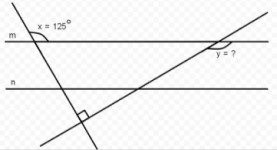
\includegraphics{April_25_Q1.jpg} Answer: \fbox{145\textdegree}}
    \item {Lines AB and CD are parallel. If $\angle EFB$ = {$(2x-100)$\textdegree} and $\angle CGF$ = {$(x+52)$\textdegree}, find the value of \angle EFB.\\
    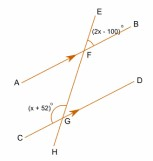
\includegraphics{April_25_Q2.jpg} Answer: \fbox{52\textdegree}}
    \item {Triangles $\bigtriangleup ABC$ and $\bigtriangleup ADC$ are inscribed in a circle and $\angle DAC$ = $\angle BCA$. Prove that $\bigtriangleup ABC$ and $\bigtriangleup ADC$ are congruent.\\
    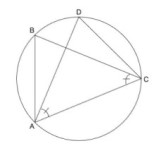
\includegraphics{April_25_Q3.jpg} \\Answer: \fbox{Use ASA: \angle $DAC$ = \angle $BCA$, both triangles share $AC$, and \angle $DCA$ = \angle $BAC$}}
    \item {A 10 m vertical lamppost ($AB$) shines light right over the head of a man who is also standing vertically. This creates a shadow on the ground right behind the person that is 1.5 times longer than his height. If the person is standing 3 m away from the lamppost, what is his height?\\
    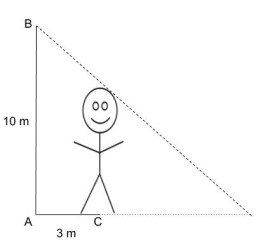
\includegraphics{April_25_Q4.jpg} Answer: \fbox{8 m}}
    \item {In right triangle $\bigtriangleup ABC$, $\angle ABC$ = {30\textdegree}, and a line is drawn from $C$ to intersect $AB$ perpendicularly at $D$. If $AB$ = 32, find the length of $CD$.\\
    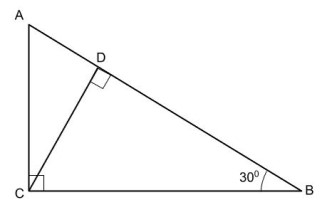
\includegraphics{April_25_Q5.jpg} Answer: \fbox{$8\sqrt{3}$}}
\end{enumerate}

\end{document}
